%DO NOT MESS AROUND WITH THE CODE ON THIS PAGE UNLESS YOU %REALLY KNOW WHAT YOU ARE DOING
\chapter*{Experimental Research}
\addcontentsline{toc}{chapter}{Experimental Research}


\section{ Beam Forming } \label{ Beam Forming } 
\noindent Figure 1 shows the beam pattern with different element spacing. Here, beam patterns with element spacing, d of $\lambda/2$, $\lambda$ and $2\lambda$ is considered and the number of elements, N is taken to be 15. Also, the incident angle, $\alpha = 0^{\circ}$. For element spacing, $d = \lambda/2$, we see that the main lobe width is large compared to when larger element spacings. Better resolution and precise location of certain sound source can be obtained with a narrower beam width. The wider the beam width, the more noise is received from the surroundings. Thus making it more difficult to identify the signal. It becomes difficult to spot the source with a wider beam width as it is more susceptible to noise received from the surroundings.

\noindent We can observe that as we increase the element spacing from $d = \lambda/2$ to $d = 2\lambda$, the main lobe width decreases, but the antenna length increases. If the element spacing is increased so that the element spacing is much greater than half a wavelength, as in the case when $d = \lambda$ and $d = 2\lambda$, the aliasing effect causes the magnitude of the side lobes to increases substantially and approach the level of the main lobe. These lobes are called grating lobes. Because of these grating lobes the antenna is equally sensitive in this direction. This is an unwanted effect. But, there are a some applications where more grating lobes are required.

\noindent Better resolution can be achieved by having longer antenna lengths. Thus there is a trade-off between the antenna length and beam width, as it is not feasible to have very long antennas. At $d = 2\lambda$, the antenna is four times longer than when $d = \lambda/2$.

\begin{figure}[h]
\centering
\subfloat[Element Spacing, $d = \lambda /2$]{
  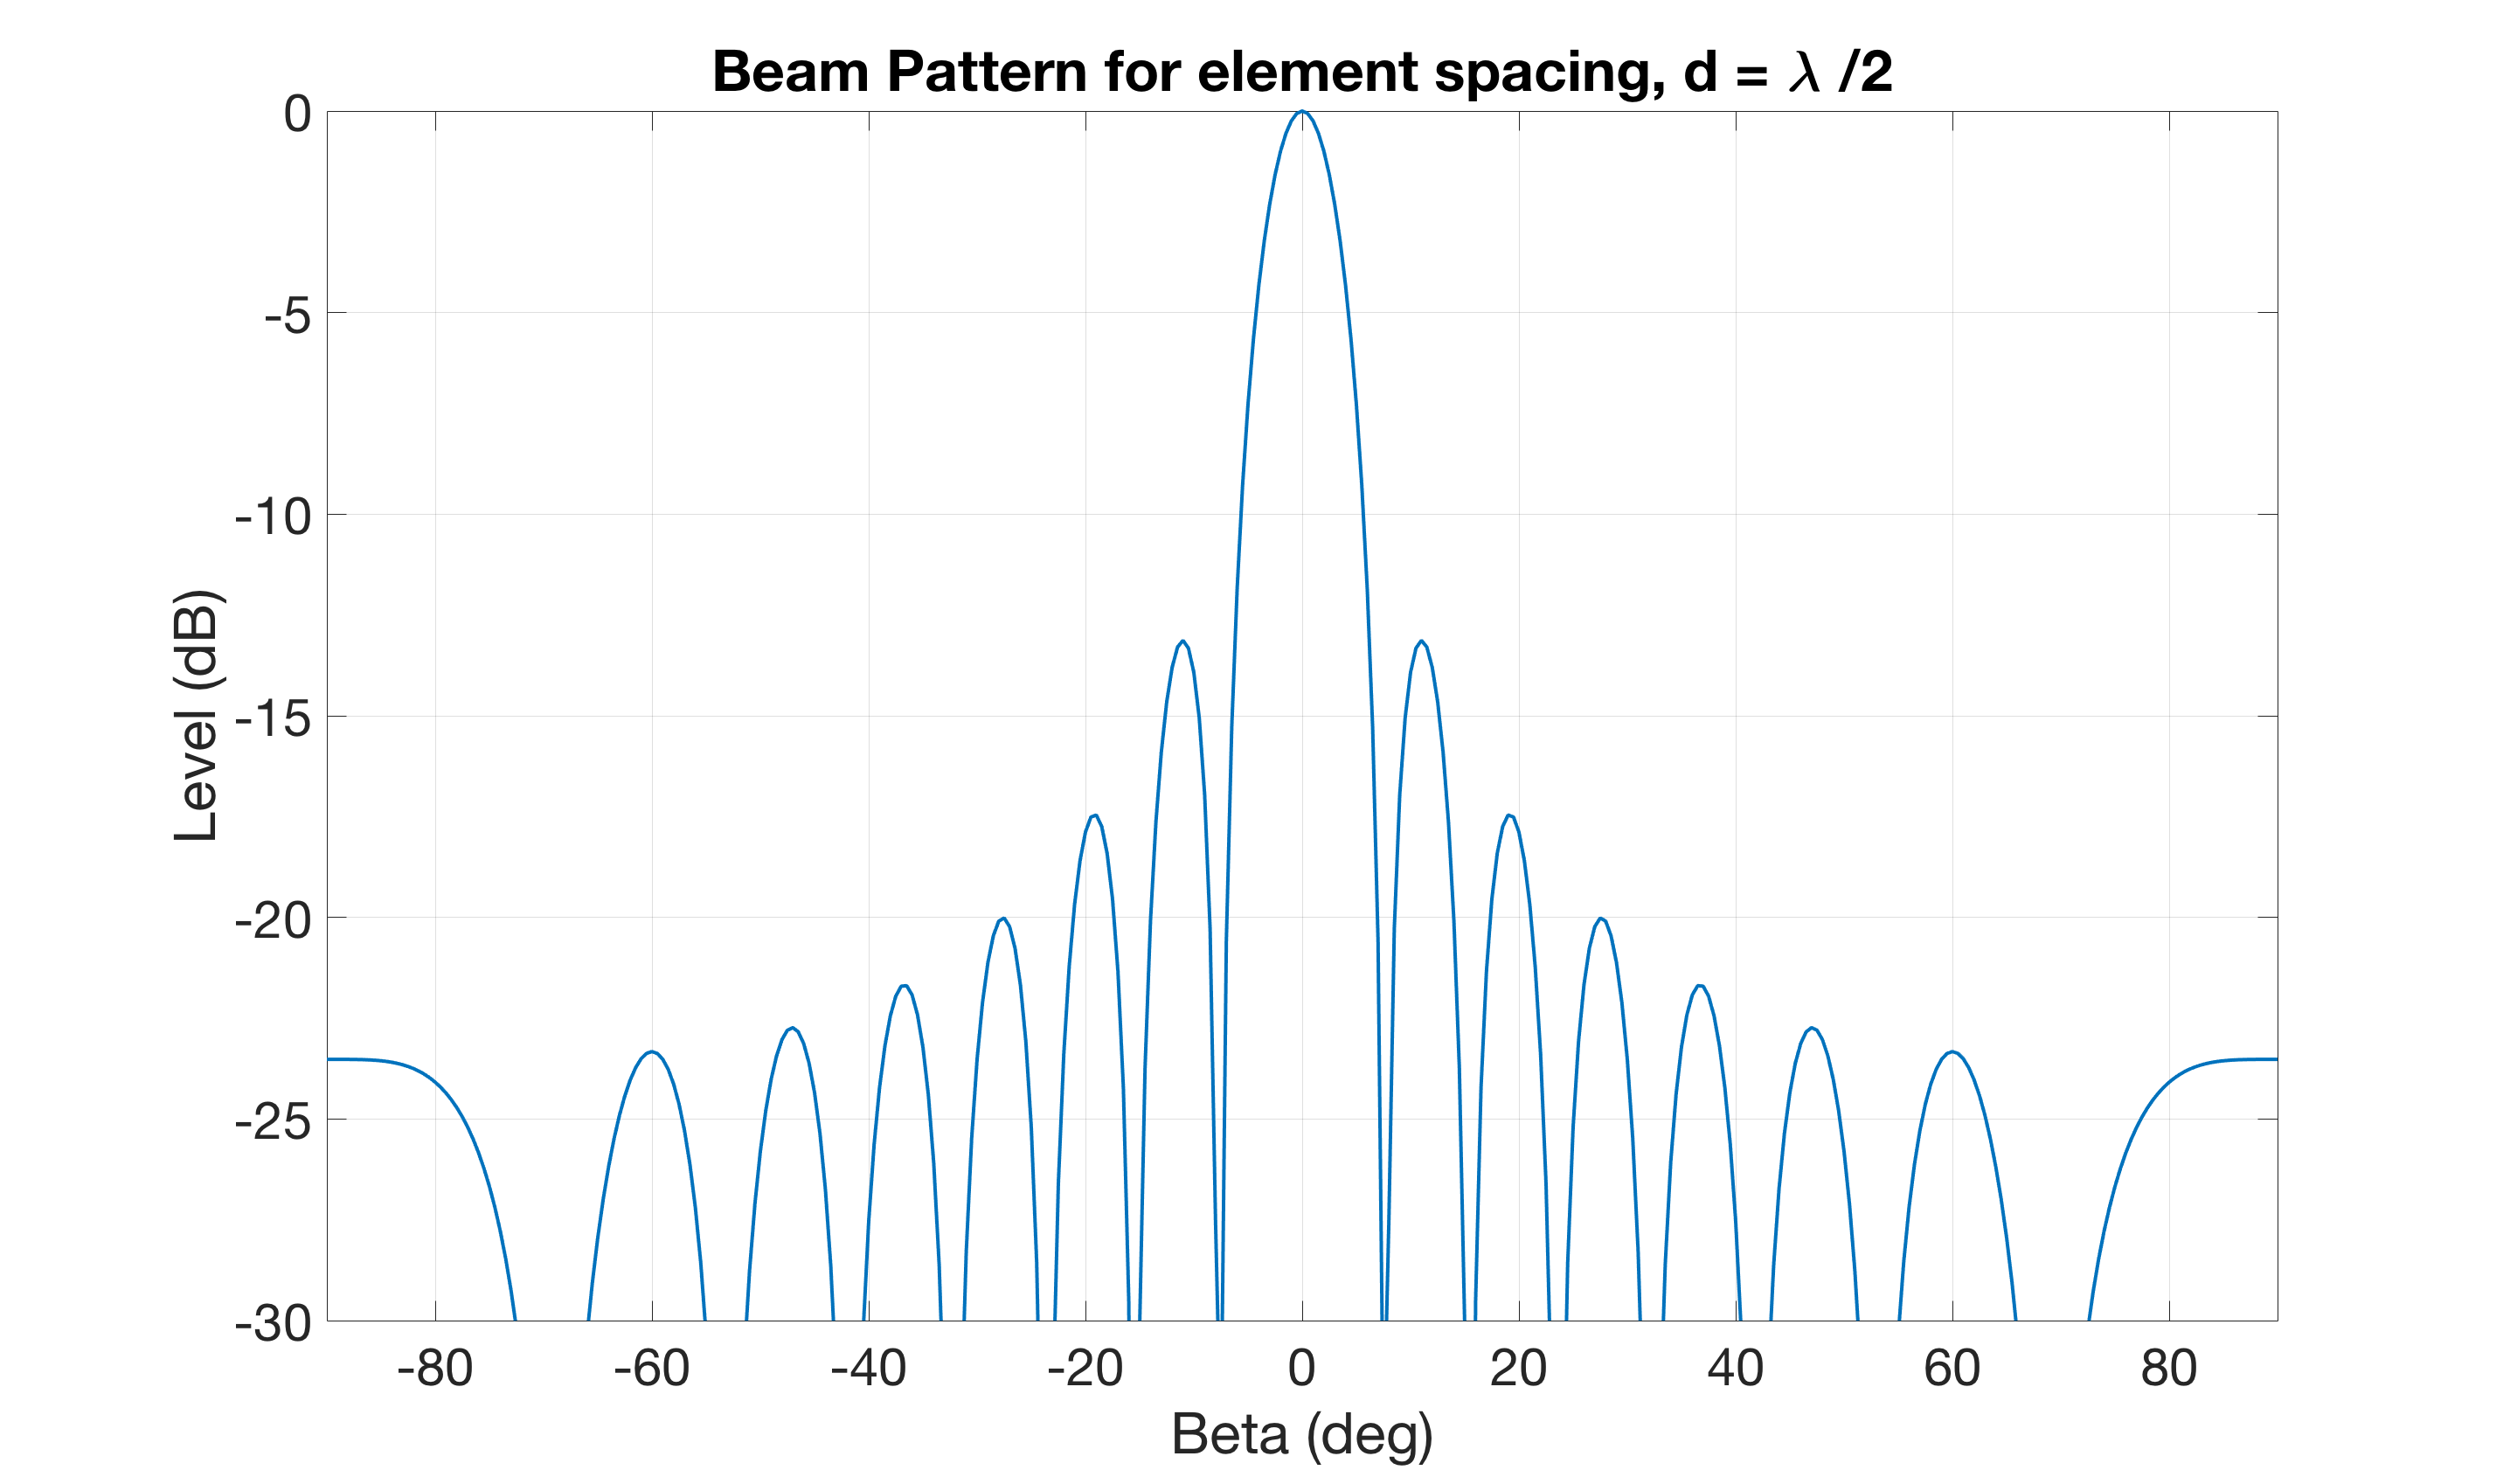
\includegraphics[width=95mm]{usp7_1.png}
}
\subfloat[Element Spacing, $d = \lambda$]{
  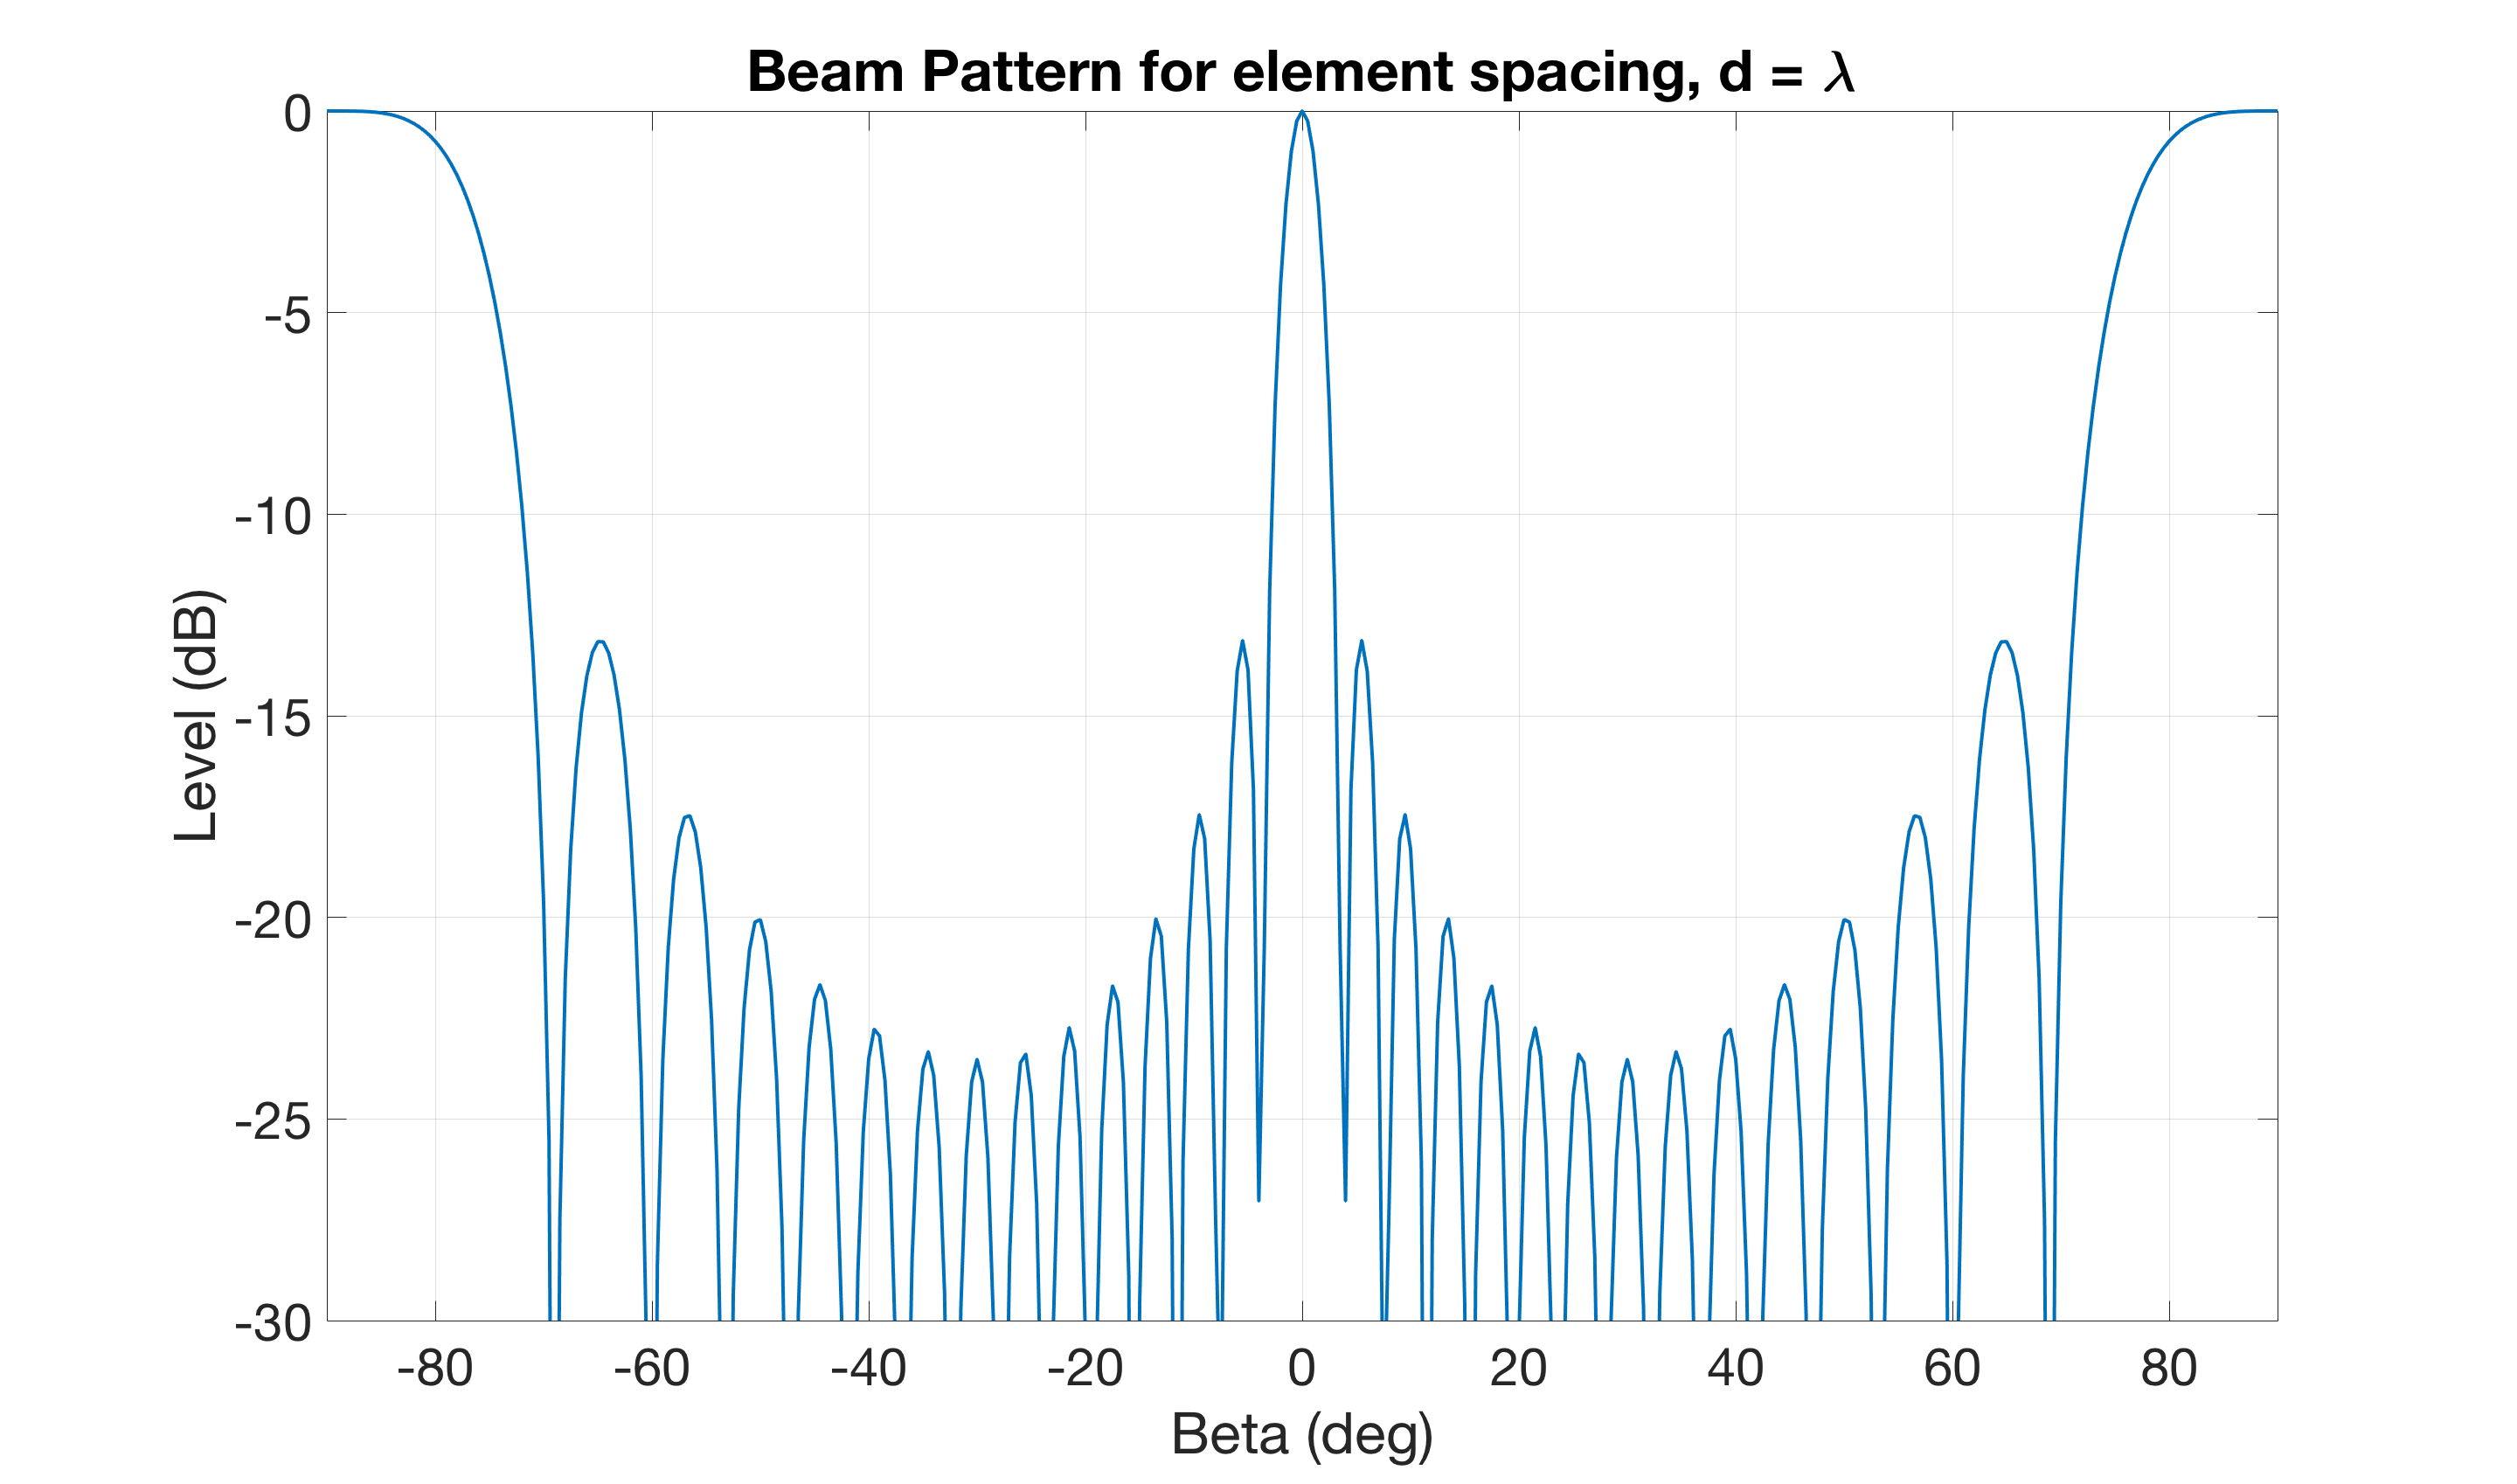
\includegraphics[width=95mm]{usp7_2.png}
}
\newline
\hbox to 18.5mm{}% !!
\subfloat[Element Spacing, $d = 2\lambda$]{
  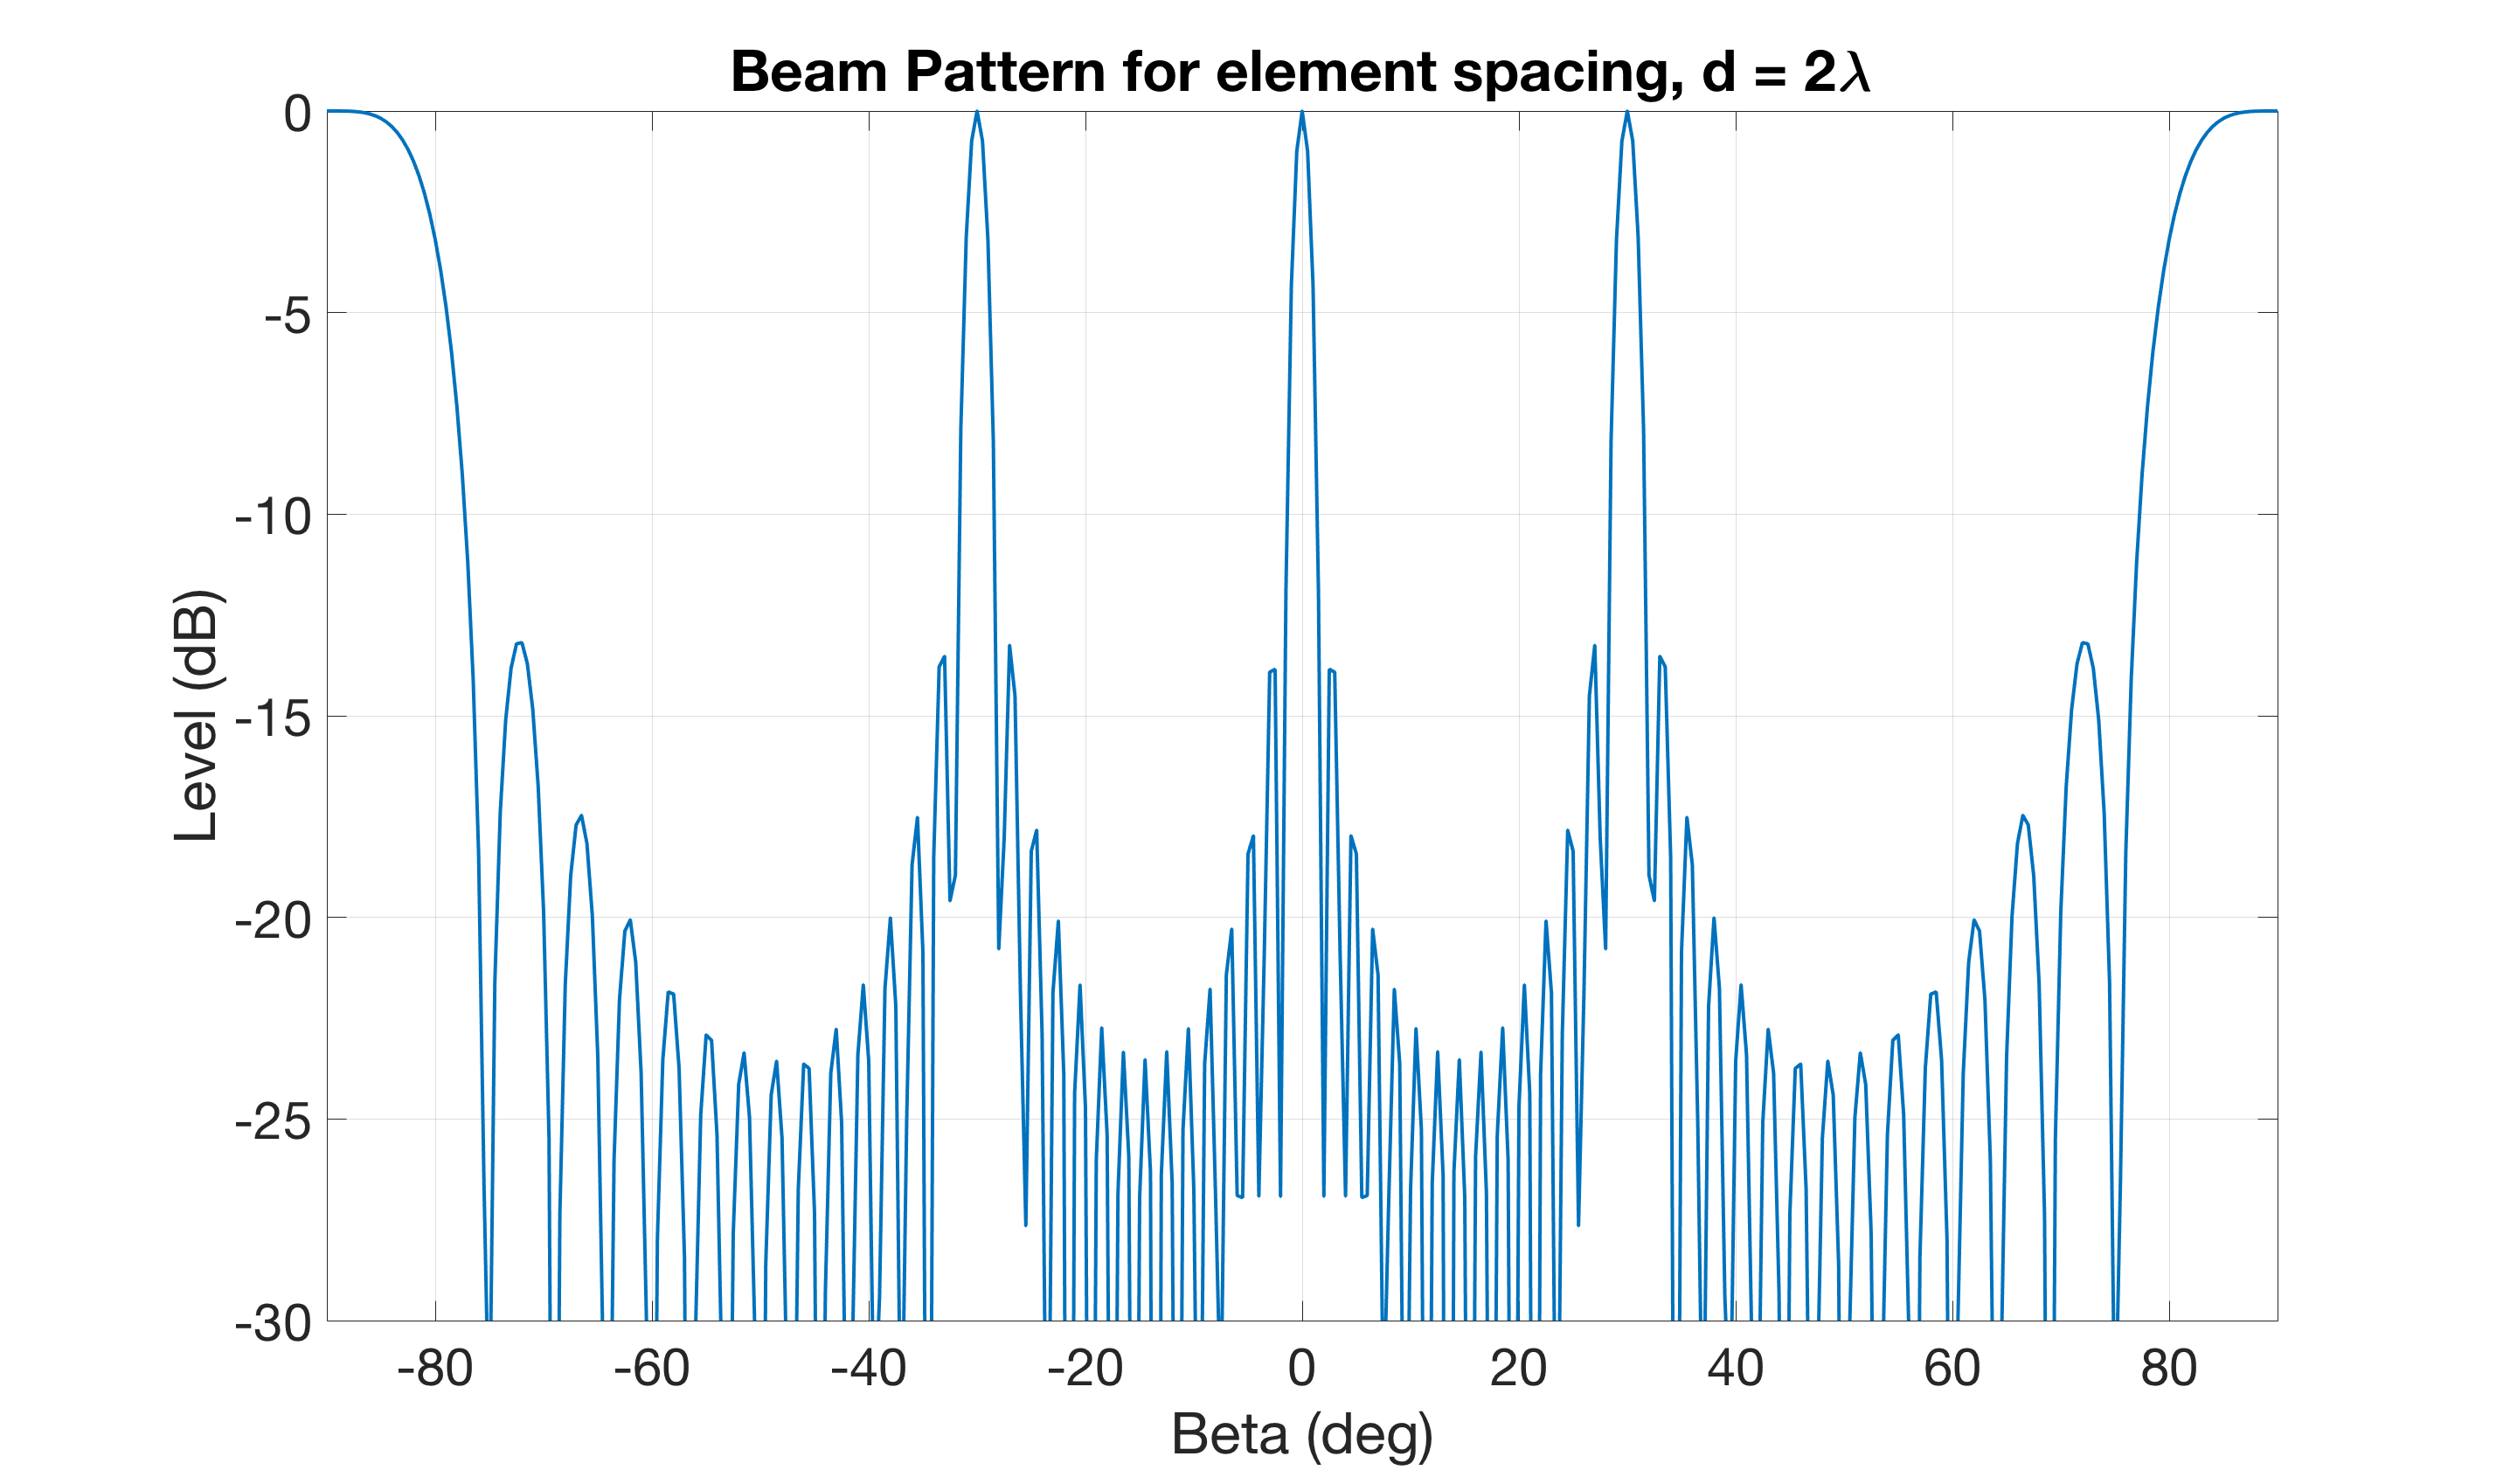
\includegraphics[width=90mm]{usp7_3.png}
}
\caption{ Beam Pattern for different Element Spacing }
\end{figure}

\newpage
\section{ Amplitude Shading } \label{ Amplitude Shading } 
\noindent Amplitude shading is an adjustment of array elements with respect to amplitude and phase. It is a convenient way to match the directivity pattern to a desired shape. It is common to employ shading as a mean to reduce the side lobe level of an antenna at the expense of the beam width of the main lobe. In most cases, amplitude shading is used to produce maximum response at the centre of the array and minimum at the ends, i.e. the sensitivity of the elements is said to be tapered from high values inside to low values outside the array. Amplitude shading is a method to suppress side lobes using window functions (example: hamming, triangular or chebychev window). There is tradeoff between beam width of main lobe and resolution.

\begin{figure}[h]
\centering
\subfloat[Element Spacing, $d = \lambda /2$]{
  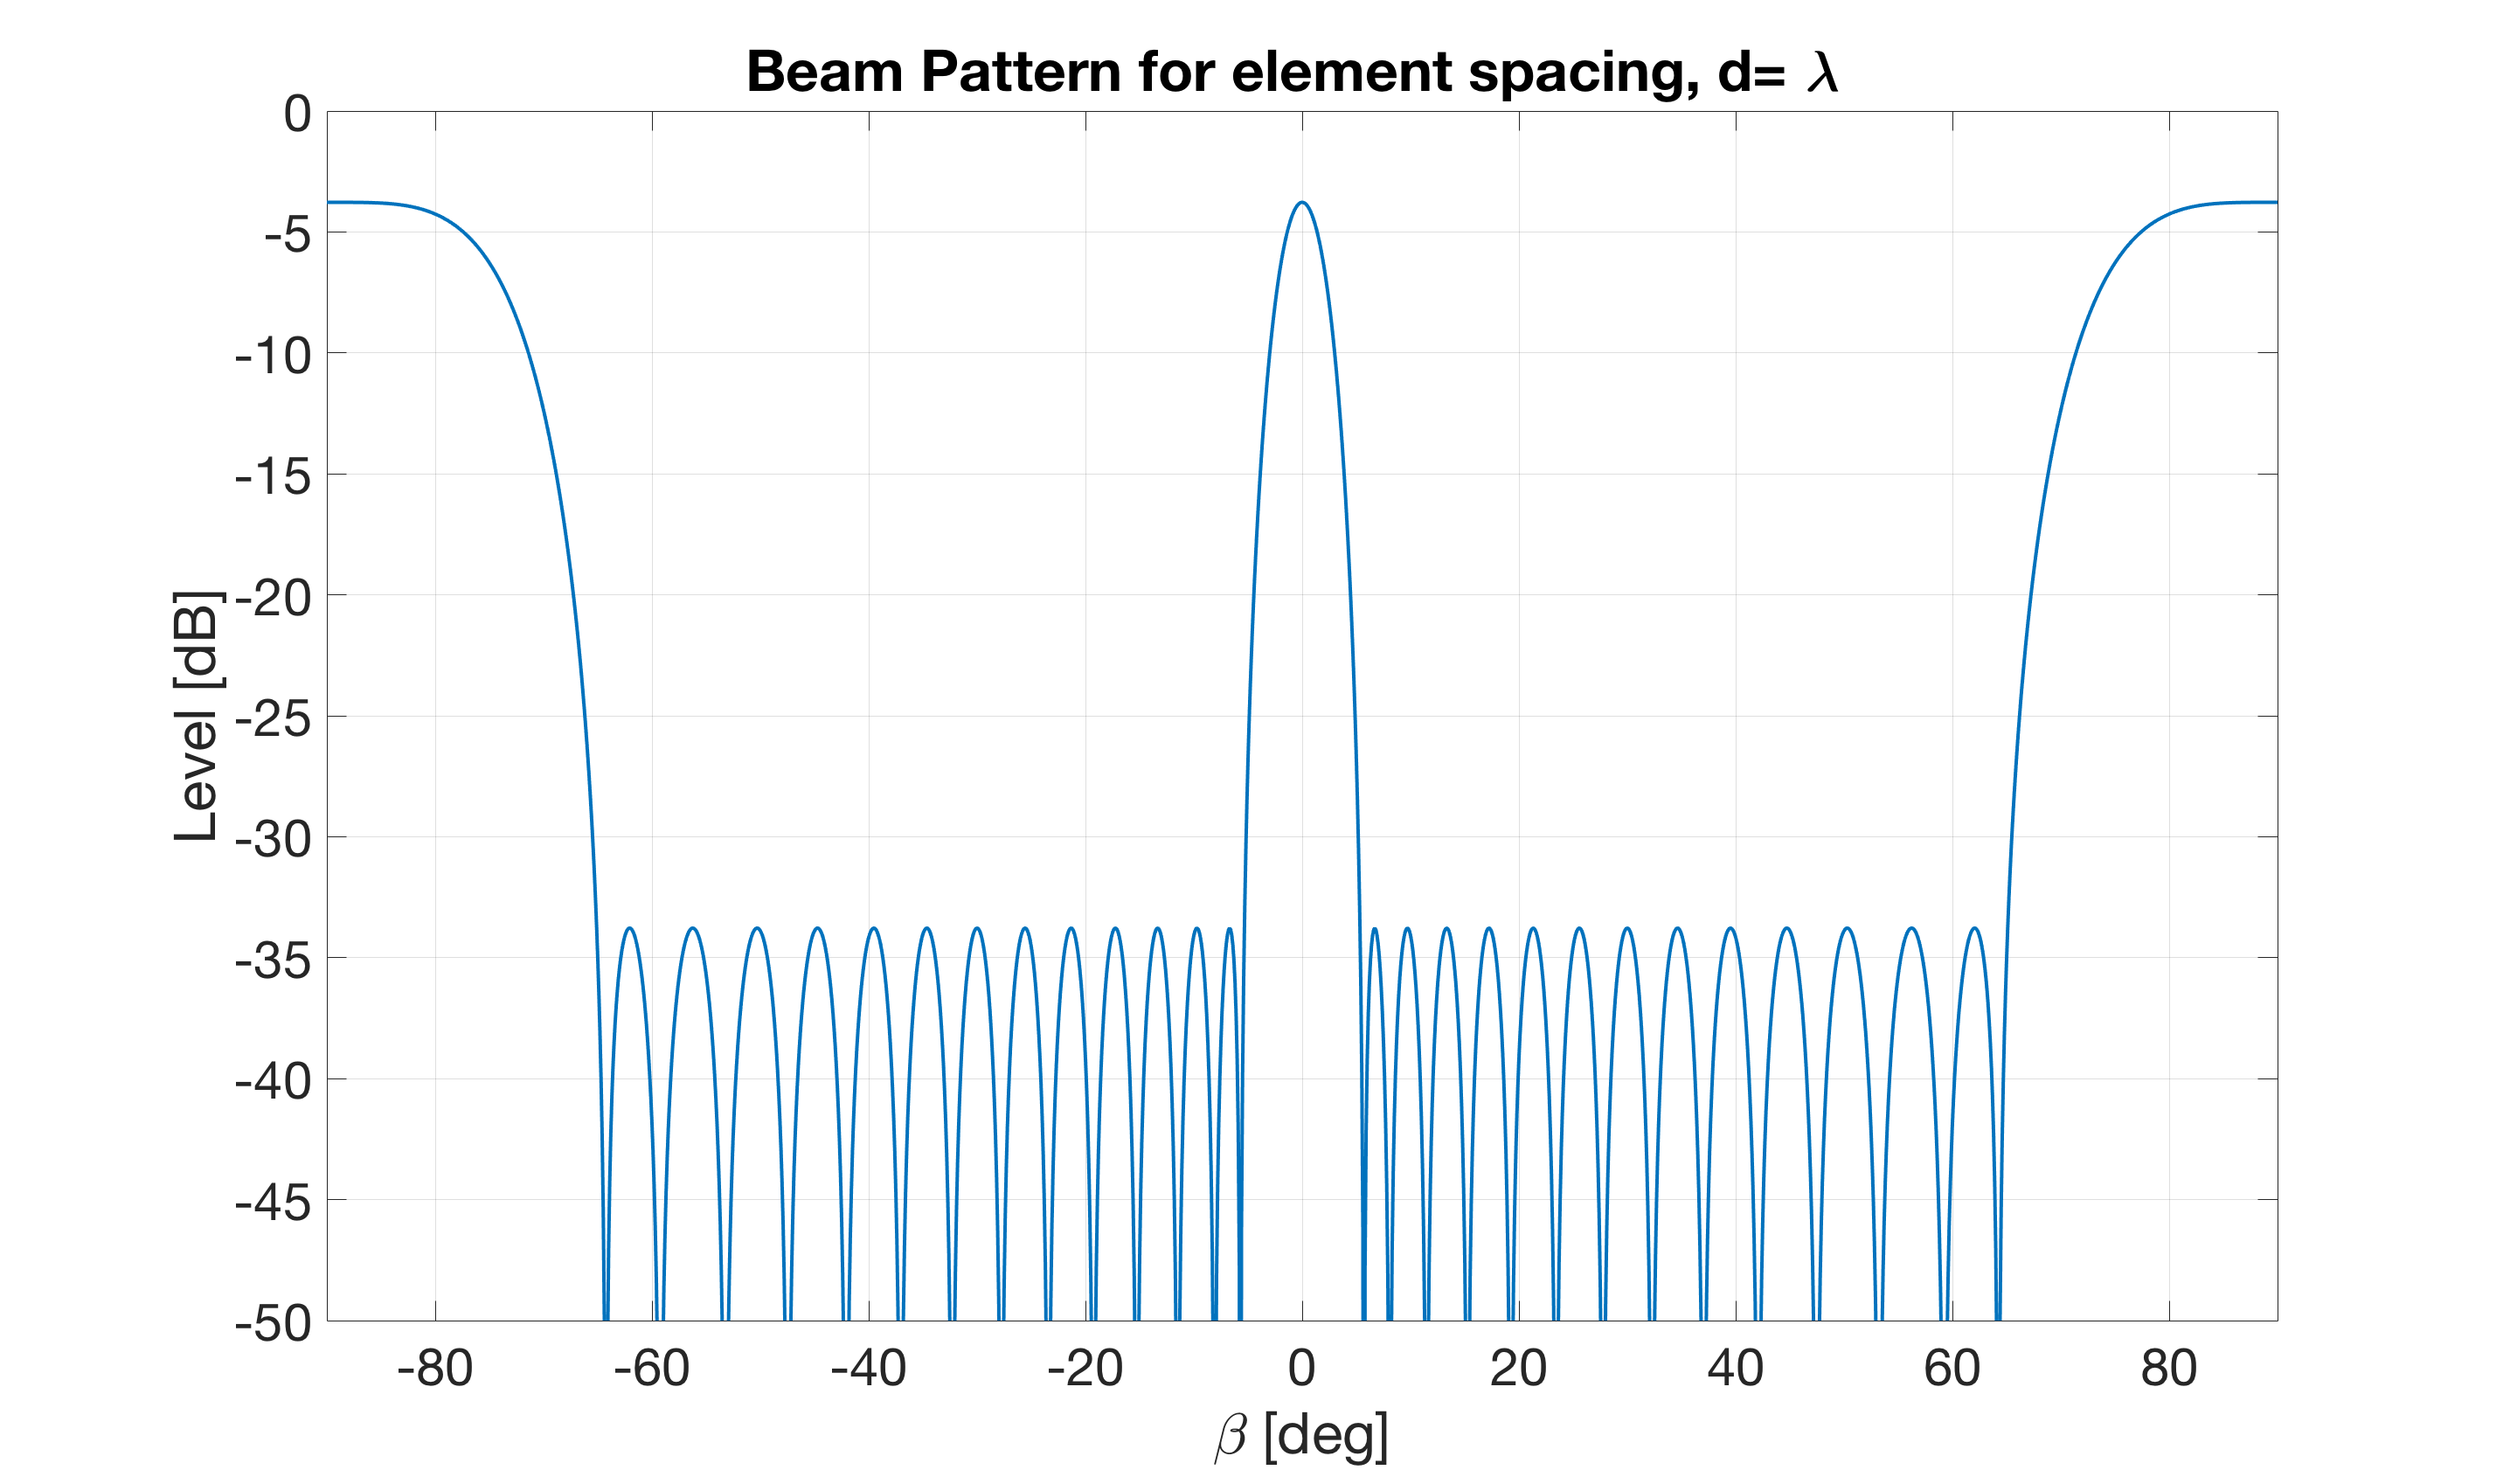
\includegraphics[width=95mm]{usp7_5.png}
}
\subfloat[Element Spacing, $d = \lambda$]{
  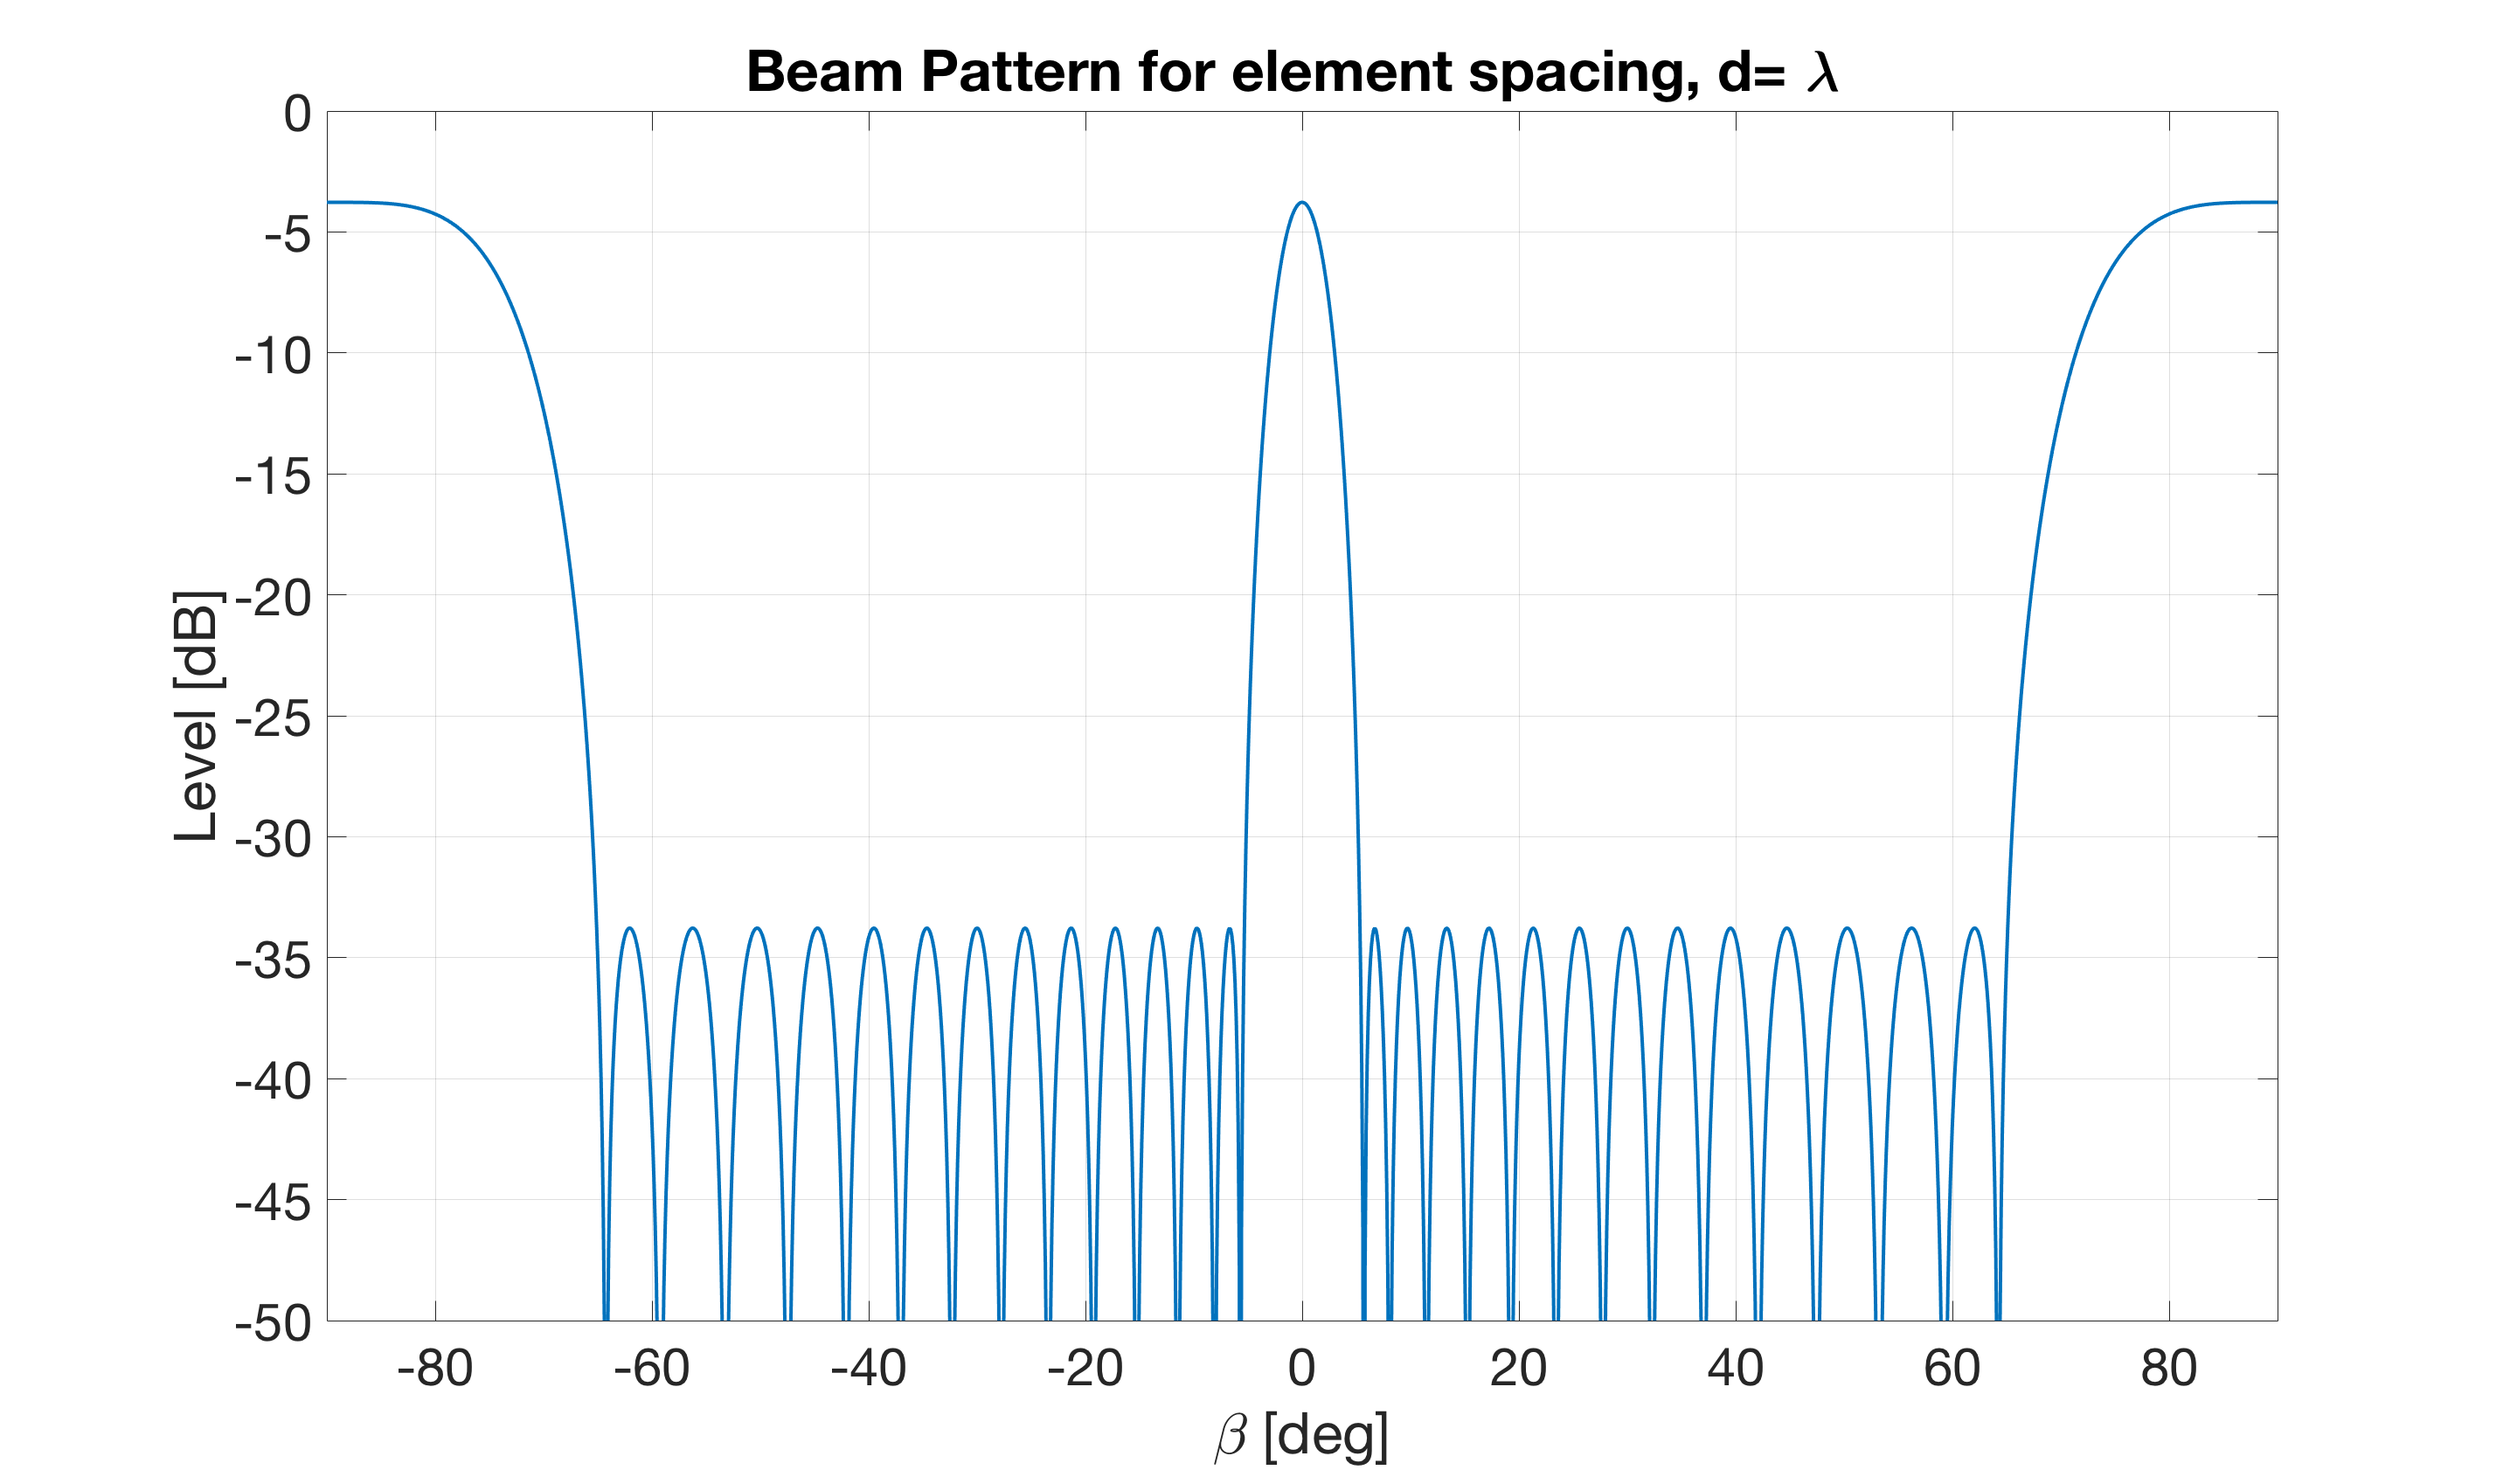
\includegraphics[width=95mm]{usp7_5.png}
}
\newline
\hbox to 18.5mm{}% !!
\subfloat[Element Spacing, $d = 2\lambda$]{
  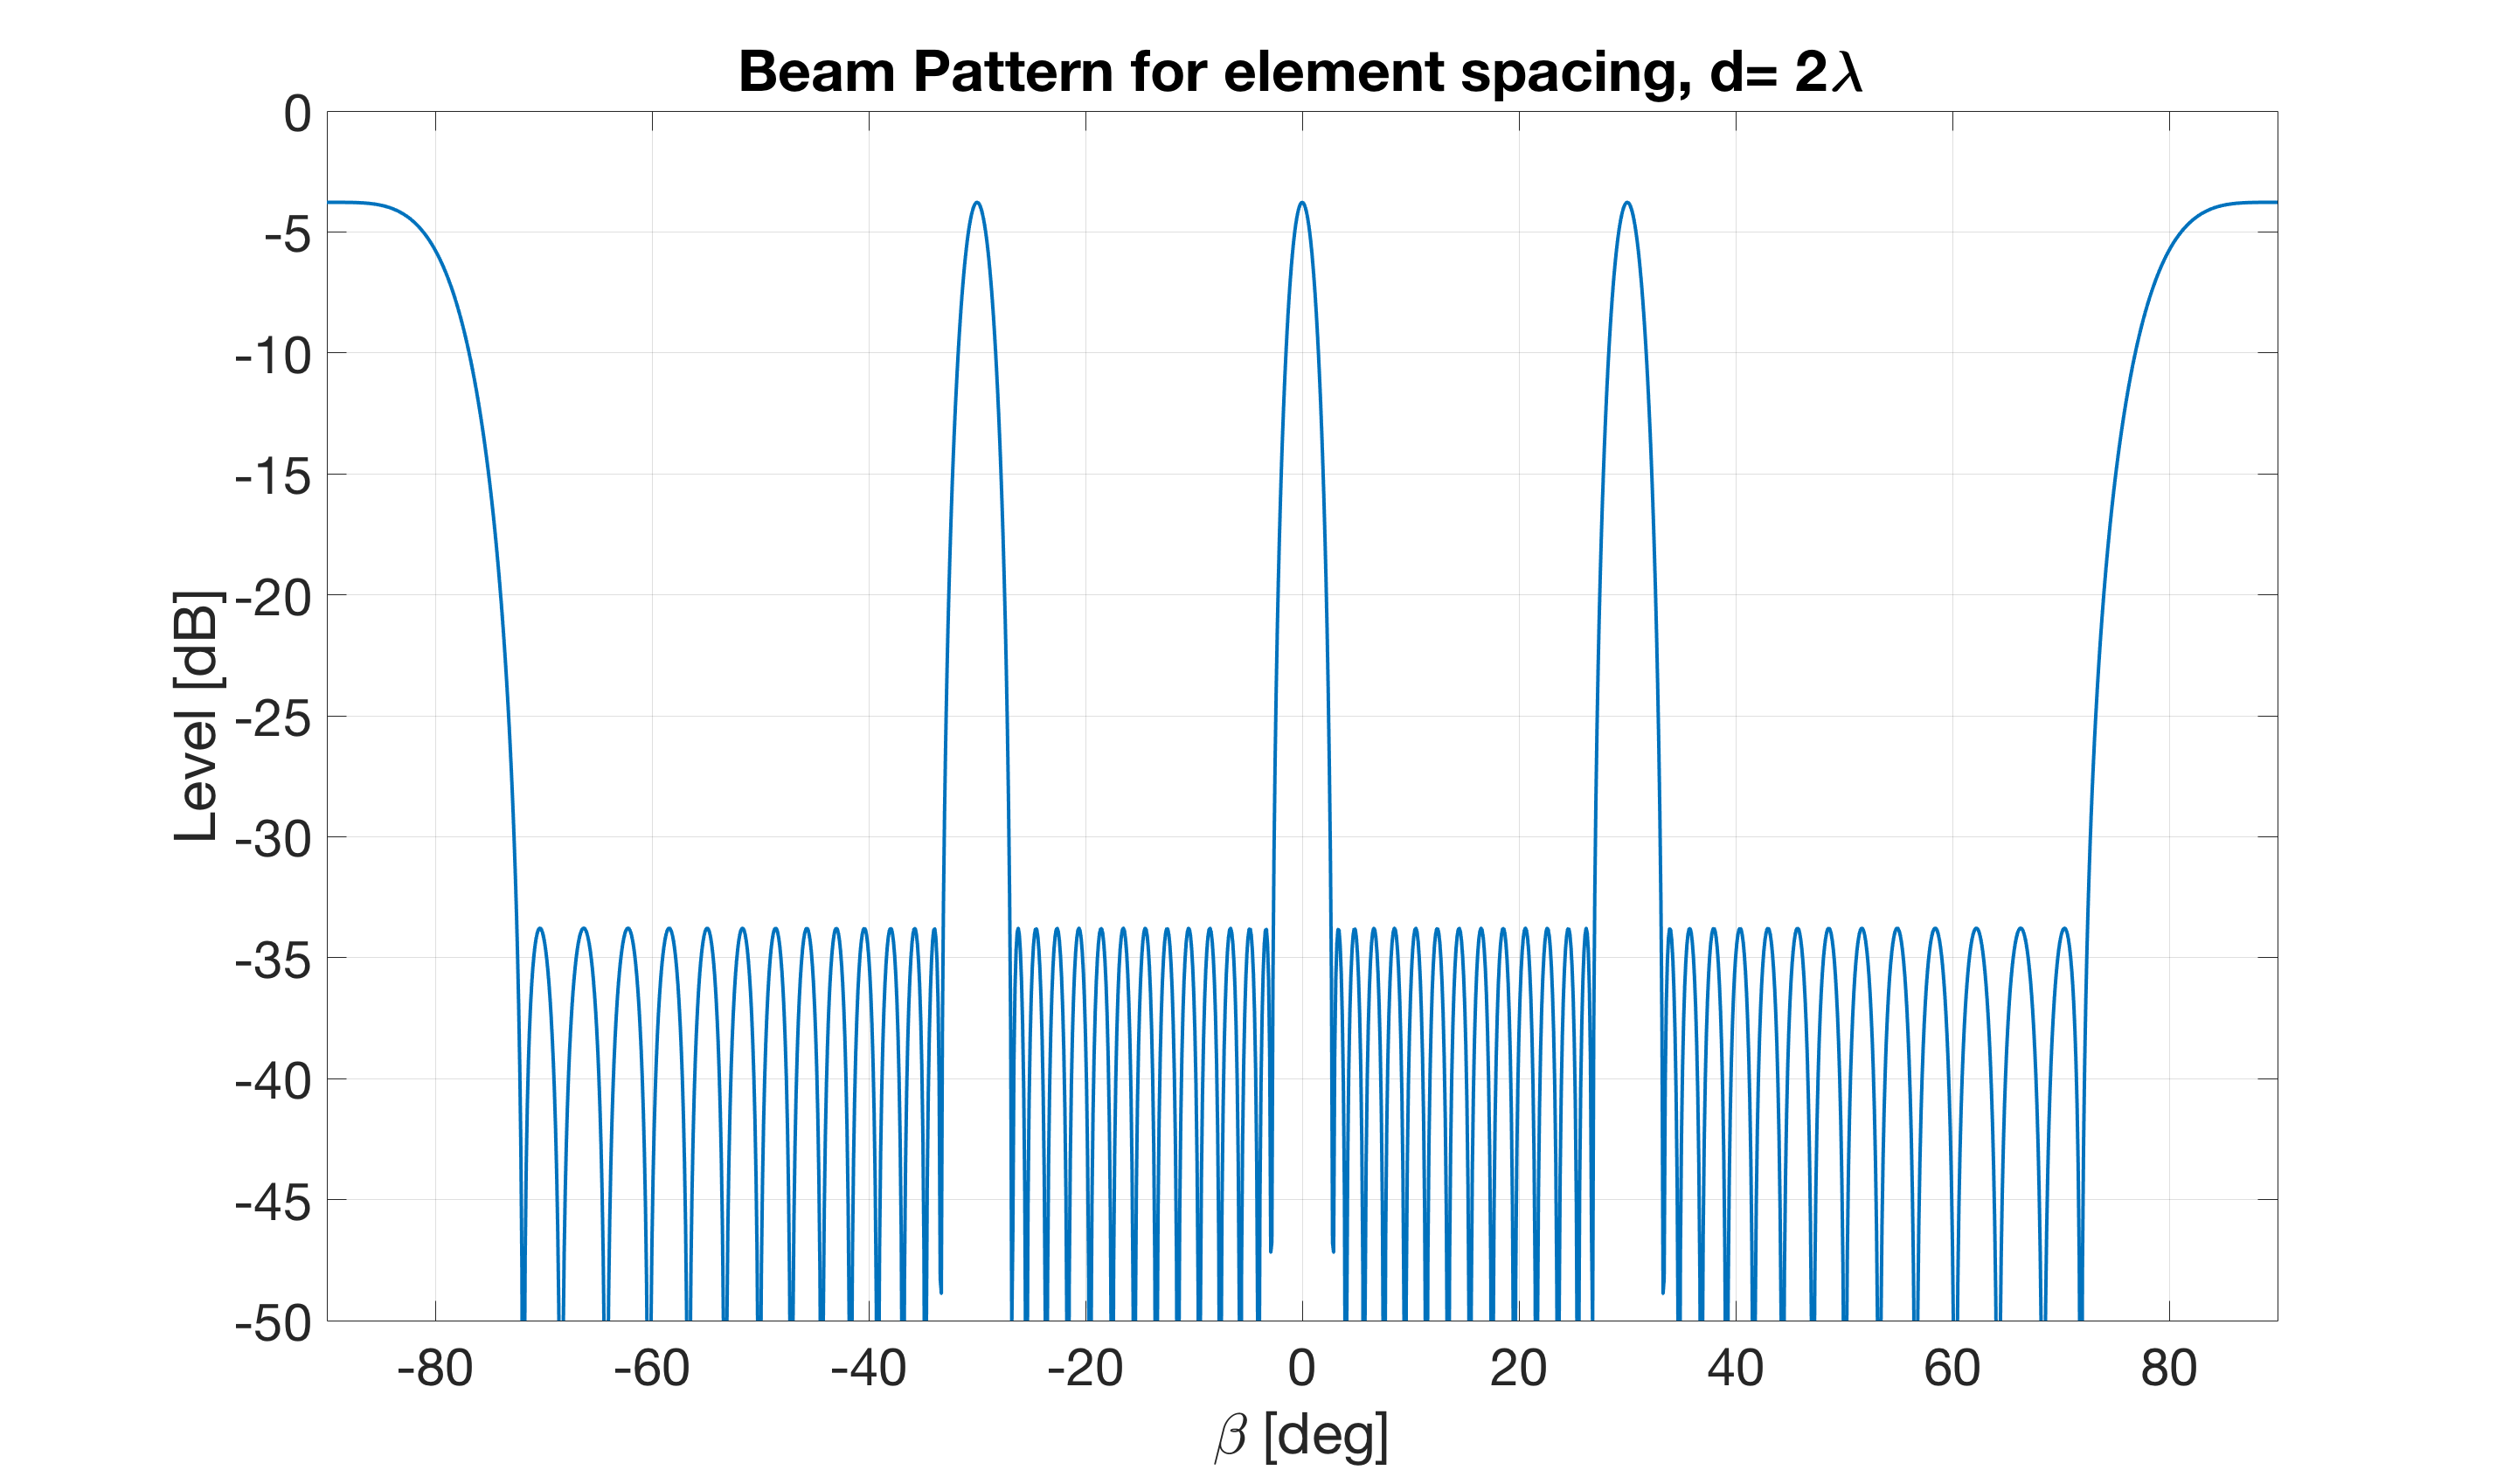
\includegraphics[width=90mm]{usp7_6.png}
}
\caption{ Beam Pattern with Amplitude Shading }
\end{figure}

\newpage

\noindent In the MATLAB code, the function, chebwin (n,r) is used to suppress the level of side lobs because we can achieve lesser beam width with better side lobe suppression as compared to the other window types. We can vary the fourier transform side lobe magnitude in chebwin function in-order to obtain different side lobe suppressions. The grating lobes are not suppressed by the chebwin window. The grating lobes can be removed by applying rectangular window on the beam pattern, which allow only main lobe to pass.

\section{ Parabolic Phase Shading (Beam Shaping) } \label{ Parabolic Phase Shading (Beam Shaping) } 

\begin{figure}[h]
\centering
\subfloat[Phase Shading]{
  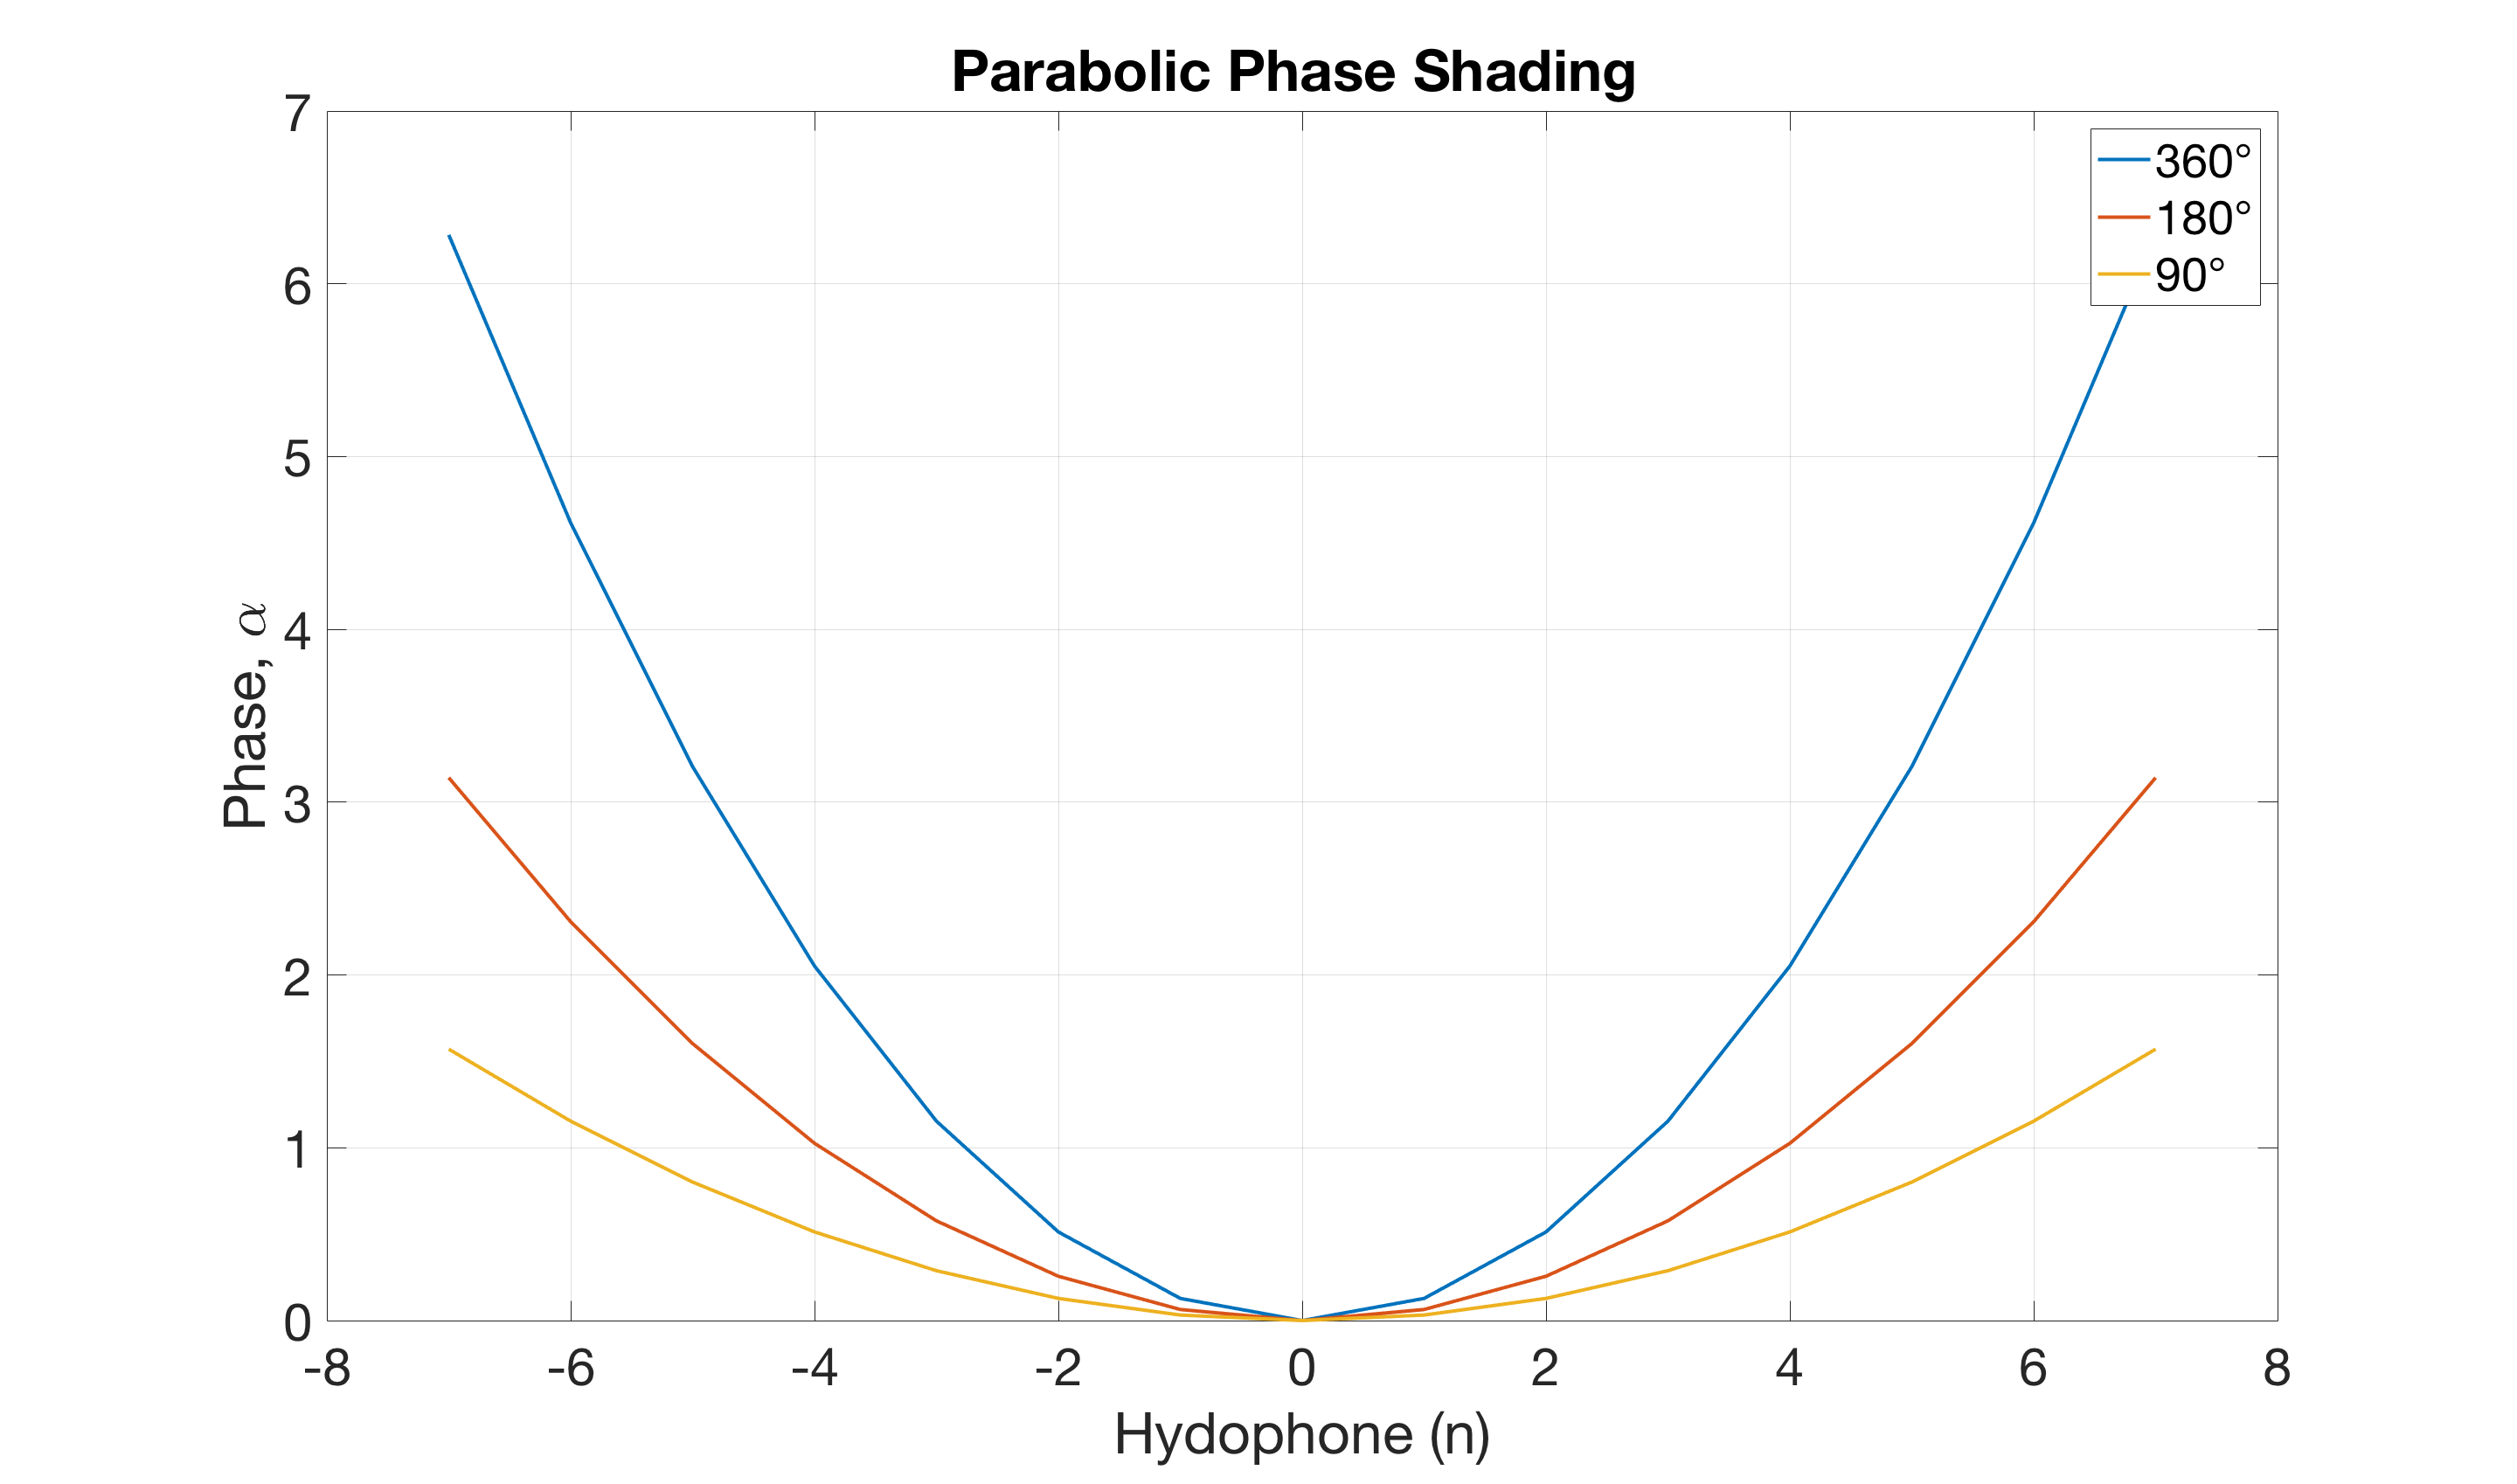
\includegraphics[width=95mm]{usp7_7.png}
}
\subfloat[Beam Pattern with Parabolic Phase Shading]{
  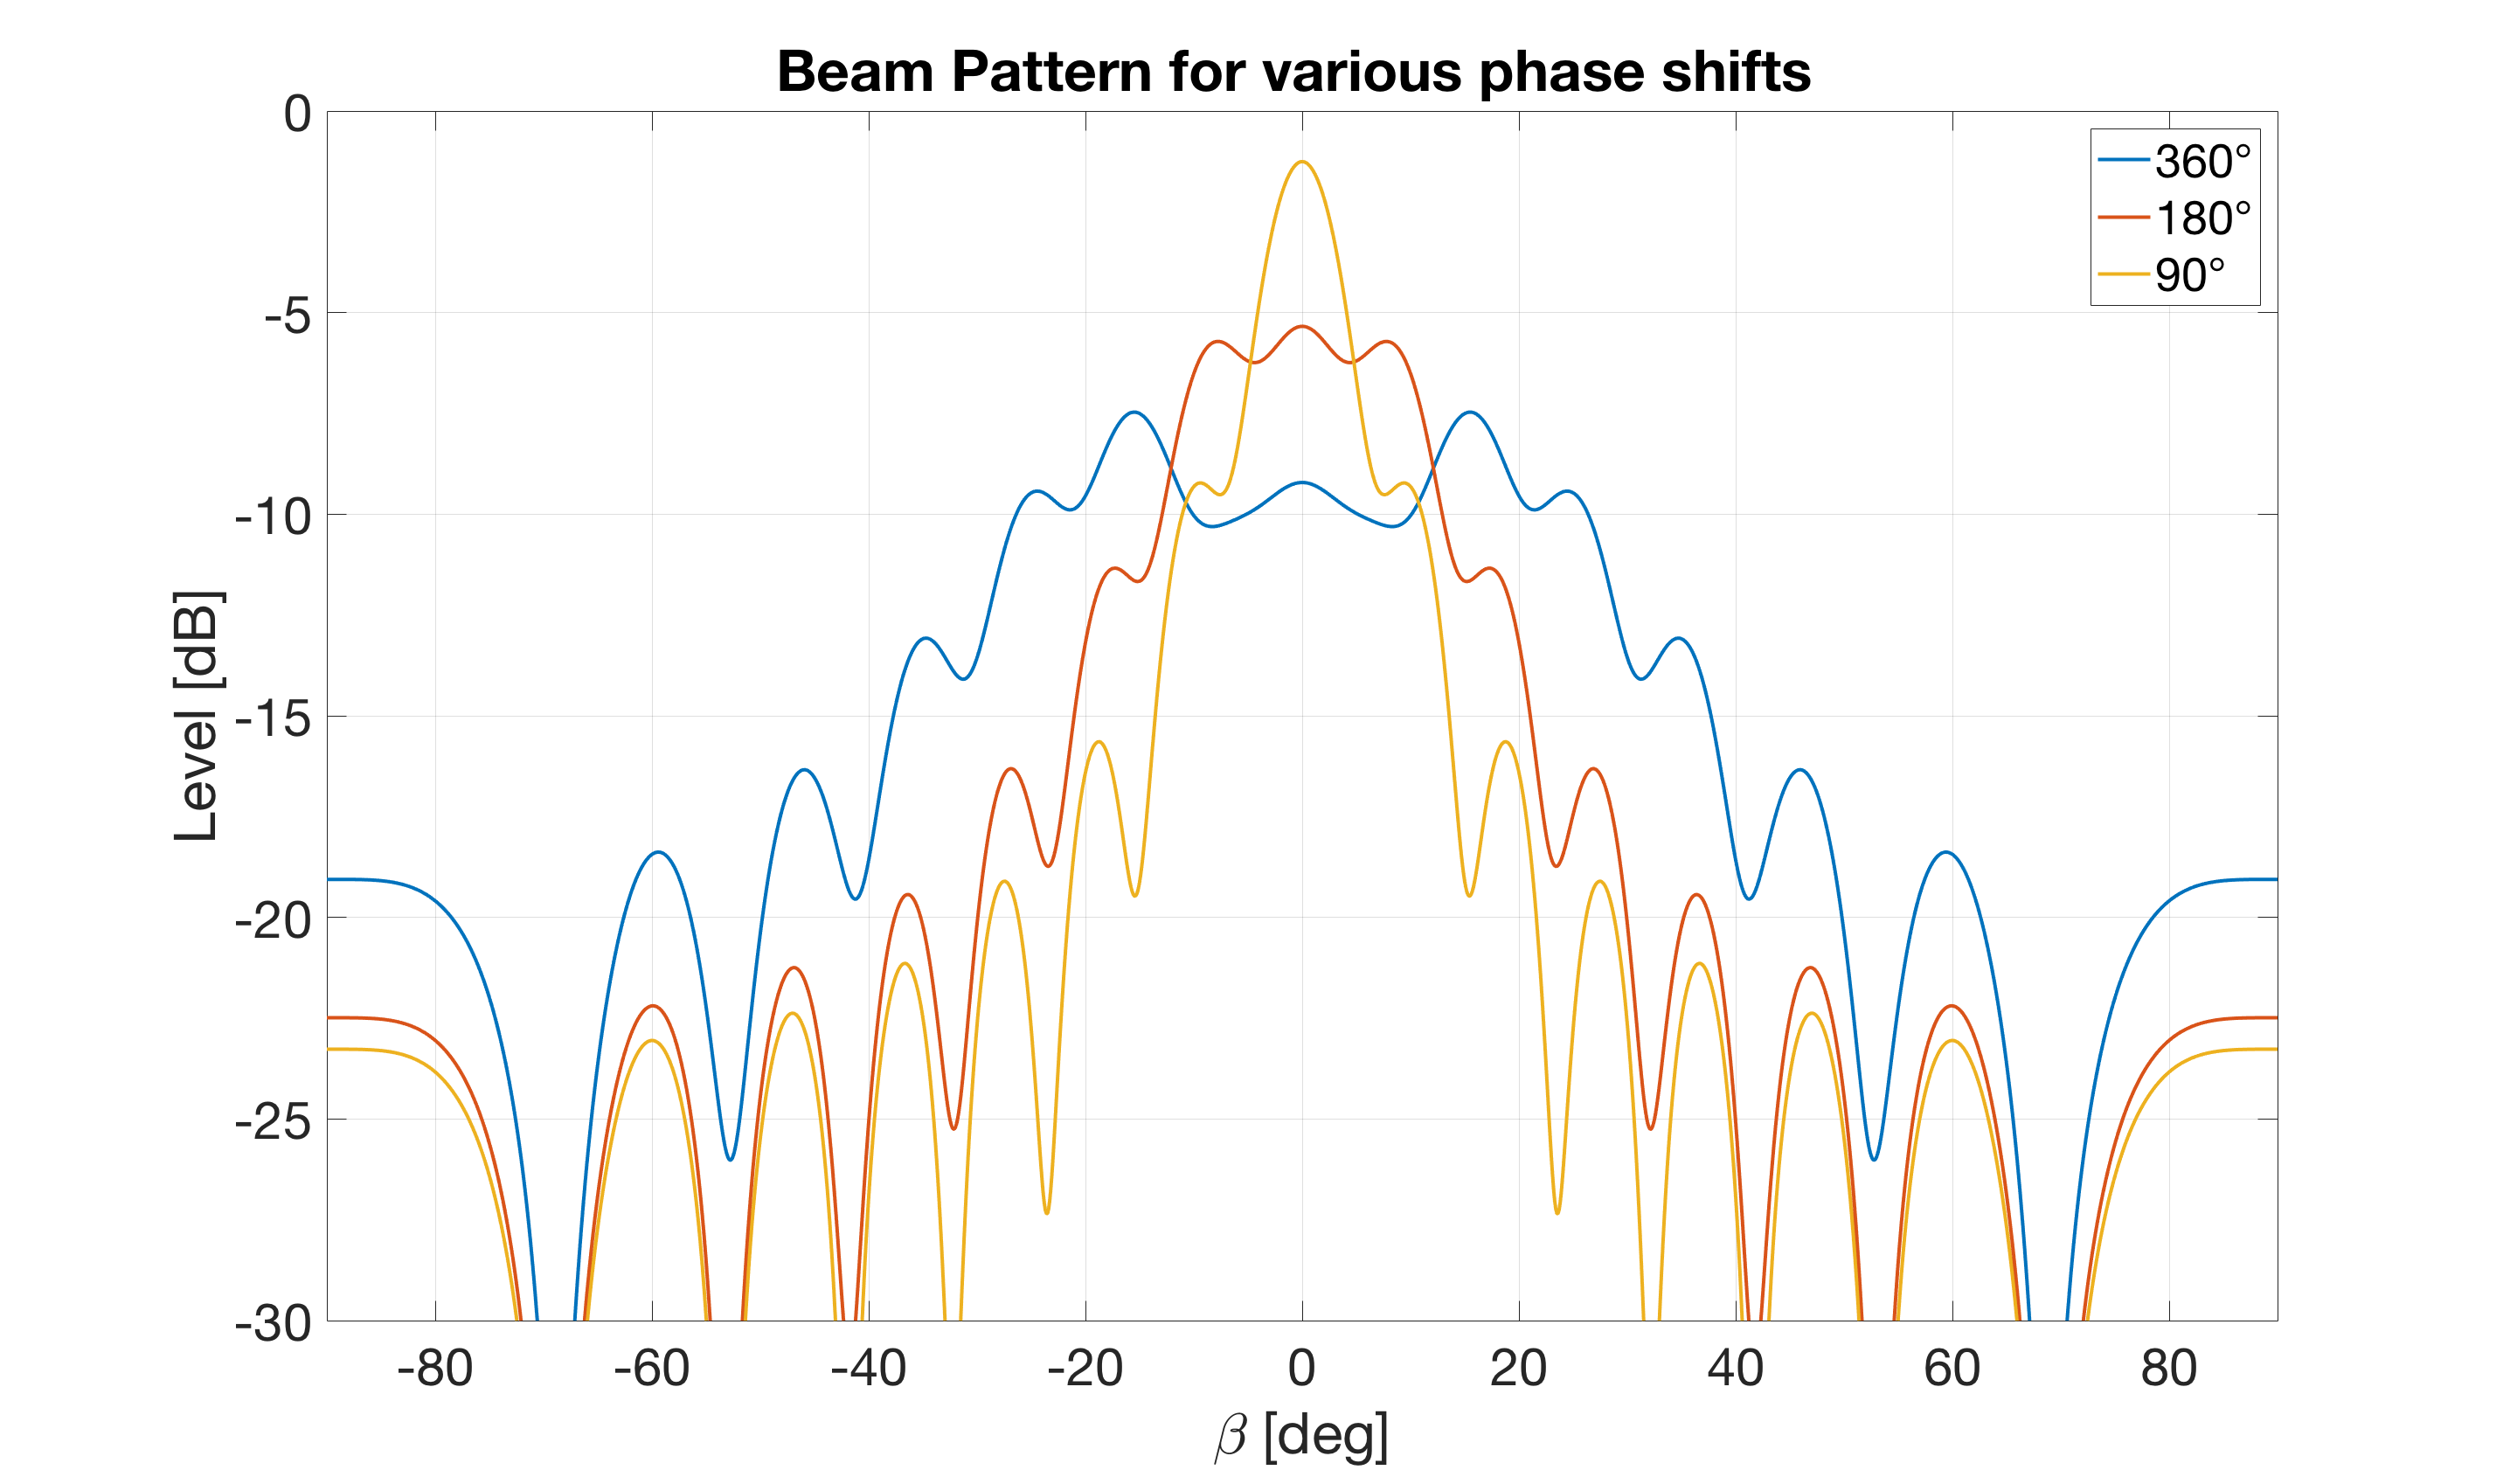
\includegraphics[width=95mm]{usp7_8.png}
}
\caption{ Parabolic Phase Shading }
\end{figure}

\noindent Beam shaping is used to design a beam pattern with a certain main lobe according to our requirements. The phase shifts of $90^{\circ}$ and $180^{\circ}$ and $360^{\circ}$ are applied to the signal fed into the transducer elements. This phase shading also provides broadening of main lobe. Many optimisations procedures are used to broaden the main beam and also suppress the side lobes to a desired level.

\noindent  As seen in Figure 3(a), it is observed that stronger the parabolic curve, stronger is the broadening of the beam. The beam pattern degrades with steeper parabolic phase which can be seen by higher side lobe levels. Also the resolution is decreased, if the beam width is increased. Figure 3(b) shows the beam pattern after parabolic phase shading.

\section{ Linear Phase Shading (Electronic Steering) } \label{ Linear Phase Shading (Electronic Steering) } 
\noindent Changing the direction of main lobe of the beam pattern is called beam steering. This is done by
changing the magnitude and phase of the hydrophones. We considered the incident angle or the steering angle to be $-20^{\circ}$, $0^{\circ}$ and $20^{\circ}$.

\noindent The summation of the signals of all the array elements/hydrophones results in the directional pattern with a maximum at the right angle $(0^{\circ})$ to the linear array or normal to the surface of the plane array. This is called the beam axial direction or broadside direction. It is possible to deflect the maximum towards other directions by mechanical or electronic steering. This procedure is called mechanical or electronic beam steering. Electronic beam steering requires the array of sensors to be composed of individually accessible elements. The device that
accomplishes the beam steering is called the beam former.
\begin{figure}[H]
\centering
{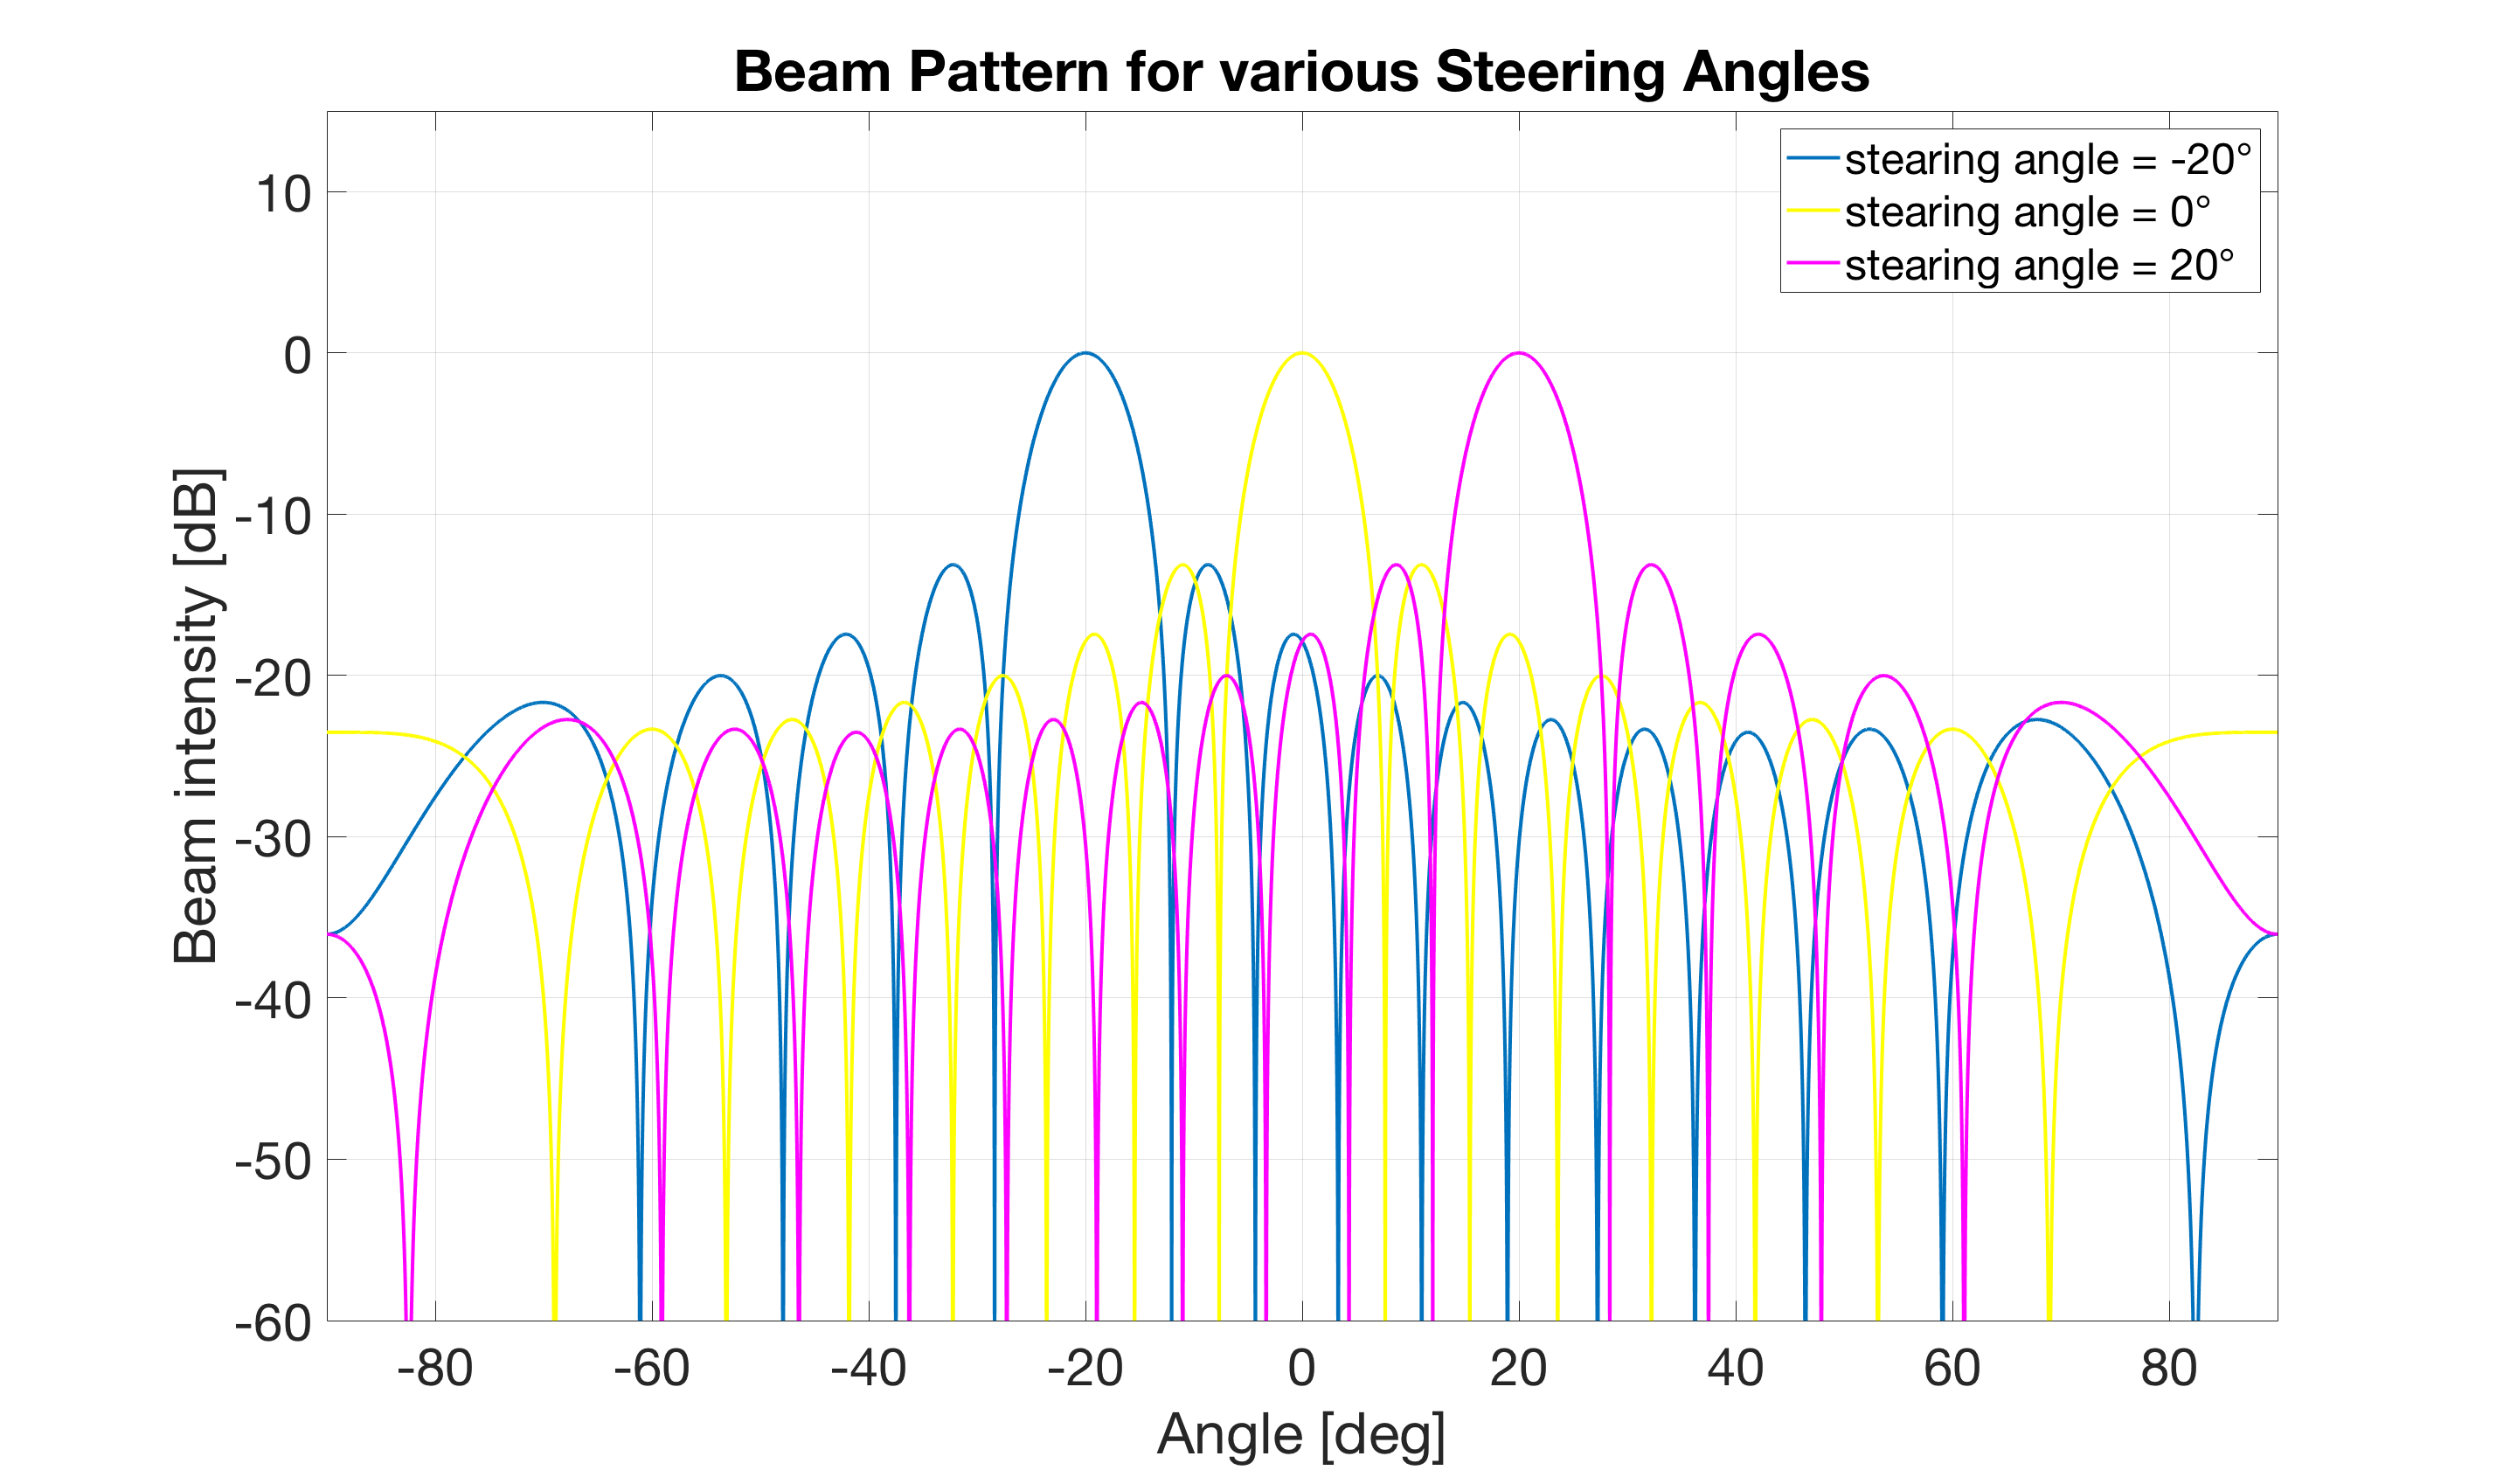
\includegraphics[scale=0.1]{usp7_9.png}}
\caption{ Linear Phase Shading }
\end{figure}

